% \documentclass[pdfCover]{myreport} % 需要pdf封面
\documentclass{myreport}
\title{数字图像频域增强实验}
\author{陈伯硕}
\date{\today}

\def\MyProject{数字图像处理}

\fancyhead{} % Clear the headers
\renewcommand{\headrulewidth}{1pt} % Width of line at top of page
\fancyhead[L]{\MyProject}
\fancyhead[R]{\MyTitle} % Mark right [R] of page with Chapter name [\leftmark]


\usepackage{subfiles}
\begin{document}

\maketitle

% \cref{fig:fish}
\begin{figure}[H]
  \centering
  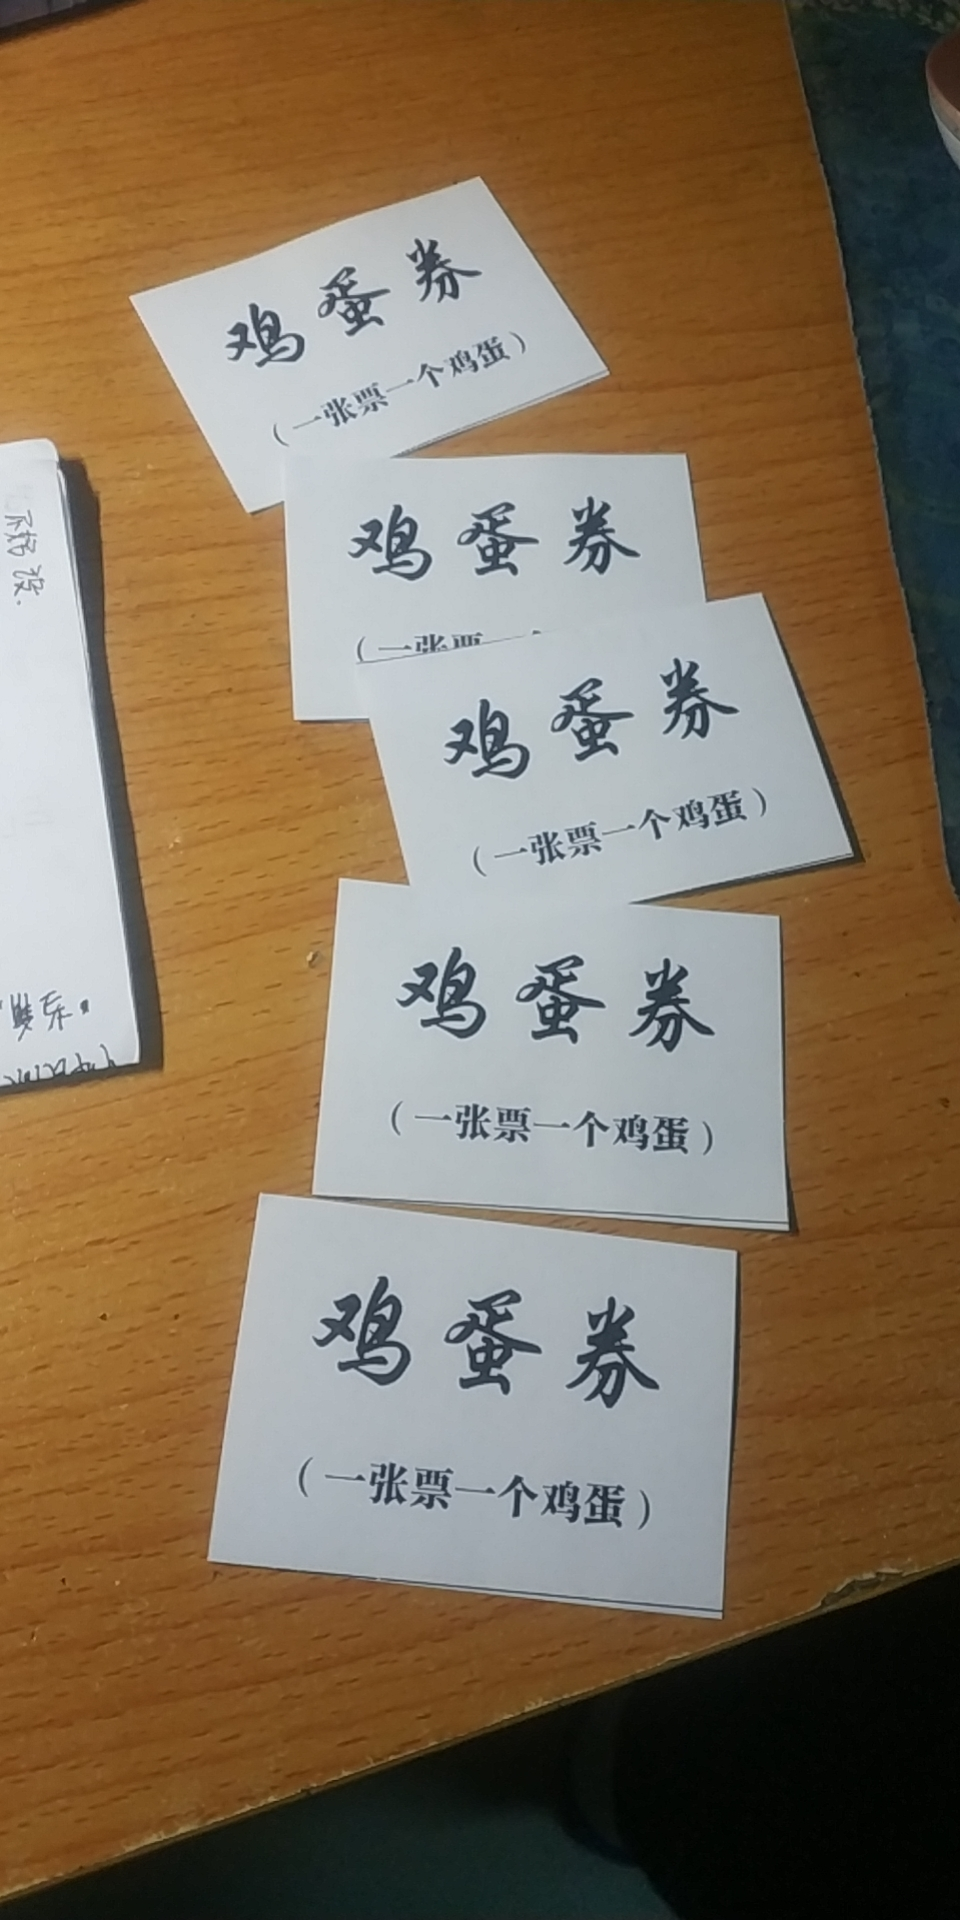
\includegraphics[width = 0.6\textwidth]{raw}
  \caption{个人手持拍照,由于灯光效果不好,有较多噪音,适合进行去噪实验}
  \label{fig:fish}
\end{figure}
\section{灰度图像的频域滤波器}
  \subsection{灰度图像进行离散傅里叶变换}
    \begin{equation}
      A_{uv} = 
      \sum_{m=0}^{M-1} \sum_{n=0}^{N-1} 
        a_{mn} \exp\left\{
          -2 \pi i \left(
            \frac{mu}{M} + \frac{nv}{N}
          \right)
        \right\}
      % \label{eq:fft2}
    \end{equation}
      % \cref{fig:freq}
      \begin{figure}[H]
        \centering
        \includegraphics[width = 0.8\textwidth]{freq}
        \caption{频率域}
        \label{fig:freq}
      \end{figure}
    \subsection{梯形低通滤波}
      \begin{equation}
        H_{uv} = \begin{cases}
        1 & D_{uv} \in (-\infty,D_0) \\
        \frac{D_{uv}-D_1}{D_0 - D_1} & D_{uv} \in (D_0, D_1) \\
        0 & D_{uv} \in (D_1,+\infty)
        \end{cases}
        % \label{eq:}
      \end{equation}
      其中
      \begin{equation}
        D_{uv} = \sqrt{u^2 + v^2}
        % \label{eq:}
      \end{equation}

      % \cref{fig:raw_mask.pdf}
      \begin{figure}[H]
        \centering
        \includegraphics[width = 0.8\textwidth]{raw_mask.pdf}
        \caption{构造数组$D(u,v)$}
        \label{fig:raw_mask.pdf}
      \end{figure}

      分段函数在python中效率不高,而且形式比较复杂
      为了计算可以使用numpy广播方式,
      引入
      \begin{equation}
        D'_{uv} = \frac{D_{uv}-D_1}{D_0 - D_1}
        % \label{eq:}
      \end{equation}
      则
      \begin{equation}
        % \label{eq:}
        H_{uv} = \begin{cases}
          1 & D' \in (1,+\infty) \\
          D'_{uv} & D' \in (0,1) \\
          0 & D' \in (-\infty,0)
        \end{cases}
      \end{equation}
      首先对$D_{uv}$线性变换,截断$D'_{uv}$即可完成变换
      \subsubsection{Case 1}
        % \cref{fig:low_pass_mask}
        \begin{figure}[H]
          \centering
          \includegraphics[width = 0.8\textwidth]{low_pass_mask}
          \caption{$D_0 = 10, D_1 = 80$}
          \label{fig:low_pass_mask}
        \end{figure}
        \begin{equation}
          A'_{uv} = A_{uv} H_{uv}
          % \label{eq:}
        \end{equation}
        % \cref{fig:low_pass_freq}
        \begin{figure}[H]
          \centering
          \includegraphics[width = 0.8\textwidth]{low_pass_freq}
          \caption{滤波后的频率域}
          \label{fig:low_pass_freq}
        \end{figure}
        \begin{equation}
          a_{xy} = \frac{1}{MN}
          \sum_{u=0}^{M-1} \sum_{v=0}^{N-1} 
            A_{uv} \exp\left\{
              2 \pi i \left(
                \frac{mu}{M} + \frac{nv}{N}
              \right)
            \right\}
          % \label{eq:fft2}
        \end{equation}
        % \cref{fig:low_pass_filter}
        \begin{figure}[H]
          \centering
          \includegraphics[width = 0.8\textwidth]{low_pass_filter}
          \caption{滤波核较小,但是保留了大部分轮廓信息,文字内容也比较清晰,没有发现明显振铃现象}
          \label{fig:low_pass_filter}
        \end{figure}
      \subsubsection{Case 2}
        % \cref{fig:ow_pass_mask_2}
        \begin{figure}[H]
          \centering
          \includegraphics[width = 0.6\textwidth]{low_pass_mask_2}
          \caption{$D_0 = 100, D_1 = 300$}
          \label{fig:ow_pass_mask_2}
        \end{figure}

        % \cref{fig:low_pass_freq_2}
        \begin{figure}[H]
          \centering
          \includegraphics[width = 0.6\textwidth]{low_pass_freq_2}
          \caption{滤波后的频率域}
          \label{fig:low_pass_freq_2}
        \end{figure}
        % \cref{fig:low_pass_filter_2}
        \begin{figure}[H]
          \centering
          \includegraphics[width = 0.6\textwidth]{low_pass_filter_2}
          \caption{图片和原图相差不大,保留了大部分信息,无振铃现象}
          \label{fig:low_pass_filter_2}
        \end{figure}
  \subsection{梯形高通滤波}
    \begin{equation}
      H_{uv} = \begin{cases}
      0 & D_{uv} \in (-\infty,D_1) \\
      \frac{D_{uv}-D_1}{D_0 - D_1} & D_{uv} \in (D_1, D_0) \\
      1 & D_{uv} \in (D_0,+\infty)
      \end{cases}
      % \label{eq:}
    \end{equation}
    \begin{equation}
      % \label{eq:}
      H_{uv} = \begin{cases}
        0 & D' \in (-\infty,0) \\
        D'_{uv} & D' \in (0,1) \\
        1 & D' \in (1,+\infty) \\
      \end{cases}
    \end{equation}

    % \cref{fig:high_pass_mask_1}
    \begin{figure}[H]
      \centering
      \includegraphics[width = 0.6\textwidth]{high_pass_mask_1}
      \caption{$D_1 = 10, D_0 = 80$}
      \label{fig:high_pass_mask_1}
    \end{figure}
    \begin{figure}[H]
      \centering
      \includegraphics[width = 0.8\textwidth]{high_pass_freq_1}
      \caption{滤波后的频率域}
      \label{fig:high_pass_freq_1}
    \end{figure}

    % \cref{fig:low_pass_filter}
    \begin{figure}[H]
      \centering
      \includegraphics[width = 0.8\textwidth]{high_pass_filter_1}
      \caption{%
        滤波核较小,文字内容也比较清晰,%
        包含噪音信息,部分纹理信息,文字边缘%
      }
      \label{fig:high_pass_filter_1}
    \end{figure}
    \subsubsection{Case 2}
        % \cref{fig:ow_pass_mask_2}
        \begin{figure}[H]
          \centering
          \includegraphics[width = 0.6\textwidth]{high_pass_mask_2}
          \caption{$D_1 = 100, D_0 = 300$}
          \label{fig:ow_pass_mask_2}
        \end{figure}

        % \cref{fig:low_pass_freq_2}
        \begin{figure}[H]
          \centering
          \includegraphics[width = 0.6\textwidth]{high_pass_freq_2}
          \caption{滤波后的频率域}
          \label{fig:low_pass_freq_2}
        \end{figure}
        % \cref{fig:low_pass_filter_2}
        \begin{figure}[H]
          \centering
          \includegraphics[width = 0.6\textwidth]{high_pass_filter_2}
          \caption{仍有边缘信息,包含较多噪音和部分纹理}
          \label{fig:low_pass_filter_2}
        \end{figure}
\section{灰度图像的离散余弦变换}
  \subsection{DCT II}
    对于一维信号,DCT 类型II
    \begin{equation}
      y_k = 2 \sum_{n=0}^{N-1} 
        x_n \cos\left(
          \frac{\pi k(2n+1)}{2N} 
        \right)
      % \label{eq:}
    \end{equation}
    % \cref{fig:dct_II_freq}
    \begin{figure}[H]
      \centering
      \includegraphics[width = 0.6\textwidth]{dct_II_freq}
      \caption{%
        DCT变换频率域,%
        默认参数使用类型II,%
        每个单元大小为$8 \times 8$%
      }
      \label{fig:dct_II_freq}
    \end{figure}

    % \cref{fig:dct_II_diff_hist}
    \begin{figure}[H]
      \centering
      \includegraphics[width = 0.6\textwidth]{dct_II_diff_hist}
      \caption{还原后的图片与原始图片的差值,
        范围在$\num{e-15}$以内,
        均值$\num{-1.21e-18}$.}
      \label{fig:dct_II_diff_hist}
    \end{figure}

    % \cref{fig:dct_II_diff}
    \begin{figure}[H]
      \centering
      \includegraphics[width = 0.6\textwidth]{dct_II_diff}
      \caption{和原图的差距图,在原图灰度大的地方相差大,正负分布总体比较偏向负数,总体差别不大}
      \label{fig:dct_II_diff}
    \end{figure}
  \subsection{DCT III}
    \begin{equation}
      y_k = 
        x_0 
        + 2 \sum_{n=1}^{N-1} 
          x_n \cos\left(
            \frac{\pi(2k+1)n}{2N}
          \right)
      % \label{eq:}
    \end{equation}
    \begin{figure}[H]
      \centering
      \includegraphics[width = 0.6\textwidth]{dct_III_freq}
      \caption{%
        DCT变换频率域,%
        参数使用类型III,%
        每个单元大小为$8 \times 8$%
      }
      \label{fig:dct_III_freq}
    \end{figure}

    % \cref{fig:dct_II_diff_hist}
    \begin{figure}[H]
      \centering
      \includegraphics[width = 0.6\textwidth]{dct_III_diff_hist}
      \caption{还原后的图片与原始图片的差值,
        范围在$\num{e-15}$以内,
        均值$\num{4.93e-17}$,
        绝对值大于DCT II.}
      \label{fig:dct_II_diff_hist}
    \end{figure}

    % \cref{fig:dct_II_diff}
    \begin{figure}[H]
      \centering
      \includegraphics[width = 0.6\textwidth]{dct_III_diff}
      \caption{和原图的差距图,
        在原图灰度大的地方相差大,
        正负分布总体比较偏向负数,
        总体差别不大}
      \label{fig:dct_III_diff}
    \end{figure}

    
\begin{appendices} % 附录
  \includepdf[pages={1},pagecommand=\section*{源代码}]{attachment/build/image_processing.pdf}
  \includepdf[pages={2-},pagecommand=\section*{\quad}]{attachment/build/image_processing.pdf}
\end{appendices}

\end{document}
